
\documentclass[14pt,a4paper,twoside,openright,nocenter,final]{extbook}
%\documentclass[12pt,b5paper,twoside,openright,final]{book}%a4paper

%\includeonly{partes/cabecera,partes/prefacio,partes/preface,partes/agradecimientos,partes/indices,partes/abbrev,partes/2services,partes/conclusions,partes/conclusiones,partes/biblio}



%%%%%%%%%%%%%%%%%%%%%%%%%%%%%%%%%%%%%%%%%%%%%%%%%%%%%%%%%%%%%%%%%%%%%%%%%%%%%%%
%%                                                                           %%
%%              Preambulo: Definicion del formato del proyecto               %%
%%                                                                           %%
%%%%%%%%%%%%%%%%%%%%%%%%%%%%%%%%%%%%%%%%%%%%%%%%%%%%%%%%%%%%%%%%%%%%%%%%%%%%%%%

%%% Paquetes para el castellano.
%\usepackage[T1]{fontenc}
%\usepackage[latin1]{inputenc}
%\usepackage[spanish]{babel}

%%% Para utilizar el entorno de Pseudocódigo

\usepackage{algorithm}
\usepackage{algorithmic}
%% Para incluir graficos
%\usepackage{graphicx}        % standard LaTeX graphics tool
\usepackage{subfigure}

\usepackage{rotating}
\usepackage{appendix}

%% Esta letra se convierte mejor a pdf que la normal
\usepackage{ae}

%%% Para las fuentes matemticas
\usepackage{amsfonts}
\usepackage{amssymb}

%%% Para hypervnculos. Compila tanto con pdflatex como con latex
%\newif\ifPDF
%\ifx\pdfoutput\undefined\PDFfalse
%\else\ifnum\pdfoutput >0\PDFtrue
%    \else\PDFfalse
%    \fi
%\fi
 
%\ifPDF
\usepackage{graphicx}
%\usepackage{pstricks} % para los dibujos del da
\usepackage{epic}           % graficos
%\usepackage{curvesls}           % curvas
% \usepackage[dvips=false,pdftex=false,vtex=false]{geometry}

\usepackage{afterpage,fancyheadings}

%\usepackage[cam,b5,center,dvips]{crop}
 
    \usepackage[pdftex]{color}
    \usepackage[pdftex]{hyperref}
%\else
%    \usepackage[dvips]{graphicx,color}
%    \usepackage[dvips]{hyperref}
%\fi
 \usepackage{ccaption}

  % Change the format of a figure caption
  % For more options see the package documentation
  \captionnamefont{\bfseries}
  \captiontitlefont{\small\sffamily}
  \captiondelim{ --- }
  \hangcaption
  \renewcommand{\figurename}{Fig.}


%% Configuracin de hyperref
\hypersetup{%
colorlinks=true,
linkcolor=black,
citecolor=black,
urlcolor=blue,
bookmarks=true,
bookmarksopen=false,
hypertexnames=false,
breaklinks=true,
pdftitle={Tesis doctoral},
pdfauthor={Juan Luis Jimenez Laredo},
%pdfkeywords={pdf, latex, tex, ps2pdf, dvipdfm, pdflatex},
bookmarksnumbered,
pdfstartview={FitH}
}%


%% Ruta de las figuras
\graphicspath{{figuras/}}

%%% Para la apariencia de las pginas
%\pagestyle{headings}
%\setcounter{secnumdepth}{10}
%\setcounter{tocdepth}{10}
%\renewcommand{\baselinestretch}{1.3}
%\setlength{\parskip}{2ex}

%%% Modificacion de los estilos de página

%\pagestyle{fancy}
%  \def\headrulewidth{0.4pt}
%  \def\footrulewidth{0.4pt}
%  \renewcommand{\chaptermark}[1]{\markboth{#1}{}}
%  \renewcommand{\sectionmark}[1]{\markright{#1}}
%  \addtolength{\headheight}{2.5pt}
%    \lhead[]{}
%    \rhead[]{}
%    \rfoot[]{\thepage}
%   \cfoot[]{}
%    \lfoot[\thepage]{}
%  \setcounter{secnumdepth}{3}
%  \setcounter{tocdepth}{3}


%\lhead[\it\thechapter]{\sl\rightmark}
%\rhead[\rm\leftmark]{\it\thesection} \rfoot[]{\thepage} \cfoot[]{}
%\lfoot[\thepage]{} \pagenumbering{arabic}



%% Para el smbolo del euro
\usepackage{eurofont}

%%% Configuramos para un tamao de papel A4
%\setlength{\paperwidth}{21cm}
%\setlength{\paperheight}{29.7cm}

%\setlength{\textwidth}{14.5cm}
%\setlength{\textheight}{23.5cm}
%\setlength{\oddsidemargin}{1.4cm}
%\setlength{\evensidemargin}{0.2cm}
%\setlength{\topmargin}{-0.2cm}

%%% Para que los vectores salgan sin flechas
\def\vec#1{\mathchoice{\mbox{\boldmath$\displaystyle#1$}}
{\mbox{\boldmath$\textstyle#1$}}
{\mbox{\boldmath$\scriptstyle#1$}}
{\mbox{\boldmath$\scriptscriptstyle#1$}}}

%% Para corregir las cabeceras largas
\newcommand{\cabecera}[2]{
\markright{\ref{#1}. \hspace{0.1ex} \MakeUppercase{#2}}}

%% Para cambiar el formato del texto de las urls
\newcommand{\texturl}[1]{\textsf{#1}}

%% Para crear urls
\newcommand{\miurl}[1]{\href{#1}{\texturl{#1}}}

%% Para cambiar el formato del texto de las tablas
\newcommand{\formatotabla}[0]{\sf \footnotesize \renewcommand{\baselinestretch}{1.1}}

\newcommand{\N}{\mathbb{N}}
%%% Para que las tablas sean tablas en vez de cuadros
%\renewcommand\listtablename{ndice de tablas}
%\renewcommand\tablename{Tabla}

\newcommand{\evag}{{\sf EvAg }}
\newcommand{\evags}{{\sf EvAgs }}
\newcommand{\evagp}{{\sf EvAg. }}
\newcommand{\evagsp}{{\sf EvAgs. }}
\newcommand{\evagc}{{\sf EvAg, }}
\newcommand{\evagsc}{{\sf EvAgs, }}



%%% Para que parta ``bien'' algunas palabras
\hyphenation {hard-ware soft-ware ins-truc-cio-nes de-sa-rro-lla-ron mo-de-lo mi-ni-mi-zar res-tric-cio-nes pa-ra-me-tros pro-ba-bi-li-dad ge-ne-ra-li-zar ge-ne-ra-li-za-cion pre-via-men-te}

%%%%%%%%%%%%%%%%%%%%%%%%%%%%%%%%%%%%%%%%%%%%%%%%%%%%%%%%%%%%%%%%%%%%%%%%%%%%%%%


\pagestyle{headings}
\setcounter{secnumdepth}{10}
\setcounter{tocdepth}{10}
\renewcommand{\baselinestretch}{1.3}
\setlength{\parskip}{2ex}


\begin{document}
%\maketitle


%%% Para que las tablas sean tablas en vez de cuadros
%\renewcommand\listtablename{ndice de tablas}
%\renewcommand\tablename{Tabla}



\thispagestyle{empty}
\begin{center}
\Large{UNIVERSIDAD DE GRANADA} \\
\bigskip
\begin{figure}[htbp]
\begin{center}

\includegraphics[width=\textwidth/2]{ugr}
\end{center}
\end{figure}
\bigskip
\bigskip


\textbf{\Large{Peer-to-Peer Evolutionary Computation: A Study of Viability}} \\
\bigskip
\bigskip
\Large{TESIS DOCTORAL} \\

\vspace{\fill}

\textbf{\Large{Juan Luis Jim\'enez Laredo}}\\
\bigskip
\Large{Granada, 2010}

\bigskip
\bigskip

\small{Departamento de Arquitectura y Tecnolog\'{\i}a de Computadores}
\end{center}


\clearpage
\thispagestyle{empty}
\begin{center}
\end{center}
\clearpage
\thispagestyle{empty}
\begin{center}

\Huge{UNIVERSIDAD DE GRANADA} \\
\bigskip
\bigskip
\bigskip

\textbf{\Large{Peer-to-Peer Evolutionary Computation: A Study of Viability}} \\
\bigskip
\bigskip
\bigskip

\textbf{\large{Memoria presentada por}} \\
\textbf{\Large{Juan Luis Jim\'enez Laredo}} \\
\bigskip



\textbf{\large{Para optar al grado de}} \\
\Large{DOCTOR EUROPEO EN INFORM\'ATICA} \\

%%%%%%%%%%%%%%%%%%%%%%%%%%%%%%%
\begin{figure}[htpb]
\begin{center}

\includegraphics[width=2.9in]{juanlusign}
\end{center}
\end{figure}
%%%%%%%%%%%%%%%%%%%%%%%%%%%%%%%
%\vspace{\fill}
\large{Fdo.  Juan Luis Jim\'enez Laredo} \\

\end{center}

\clearpage
\thispagestyle{empty}
\begin{center}
\end{center}
\clearpage

\thispagestyle{empty}
\bigskip
\textbf{D. Juan Juli\'an Merelo Guerv\'os}, Catedr\'atico de Universidad y \textbf{D. Pedro A. Castillo Valdivieso}, Profesor Titular de Universidad, ambos del Departamento de Arquitectura y Tecnolog\'{\i}a de Computadores de la Universidad de Granada\\
\\
\\
\textbf{CERTIFICAN} \\
\\
\\
Que la memoria titulada: \emph{``Peer-to-Peer Evolutionary Computation: A Study of Viability''} ha sido realizada por \textbf{Juan Luis Jim\'enez Laredo} bajo nuestra direcci\'on en el Departamento de Arquitectura y Tecnolog\'{\i}a de Computadores de la Universidad de Granada para optar al grado de Doctor en Inform\'atica. \\
\\
\medskip
\hspace{\fill}Granada, a 26 de Abril de 2010 \\

%%%%%%%%%%%%%%%%%%%%%%%%%%%%%%%
\begin{figure}[htpb]
\begin{center}
\subfigure{
\includegraphics[width=2.3in]{pedrosign}}
\hspace{4pt}
\subfigure{
\includegraphics[width=2.3in]{jjsign}} 
\end{center}
\end{figure}
%%%%%%%%%%%%%%%%%%%%%%%%%%%%%%%

%\vspace{\fill}

\begin{center}
\begin{tabular}{cc}
Fdo. Pedro A. Castillo Valdivieso   &    Juan Juli\'an Merelo Guerv\'os  \\
Director de la Tesis  & Director de la Tesis
\end{tabular}
\end{center}


\pagenumbering{roman}
\pagenumbering{arabic}

%\end{document}                     % Eliminarlo al compilar el documento maestro, ponerlo para compilarlo separado



%%%%%%%%%%%%%%%%%%%%%%%%%%%%%%%%%%%%%%%%%%%%%%%%%%%%%%%%%%%%%%%%%%%%%%%%%%%%%%%
%%                                                                           %%
%%                                   Indice                                  %%
%%                                                                           %%
%%%%%%%%%%%%%%%%%%%%%%%%%%%%%%%%%%%%%%%%%%%%%%%%%%%%%%%%%%%%%%%%%%%%%%%%%%%%%%%

\frontmatter
%\documentclass[12pt,a4paper,twoside]{book} 
\usepackage[spanish]{babel} % de pedro
\usepackage{graphics,graphicx,epsfig,color,float,afterpage,fancyheadings,subfigure,moreverb,alltt} % de pedro
\usepackage[latin1]{inputenc} % tildes de pedro

\usepackage{algorithm}
\usepackage{algorithmic}

\usepackage{rotating}
\usepackage{url}

%% Esta letra se convierte mejor a pdf que la normal
\usepackage{ae}

%%% Para las fuentes matemticas
\usepackage{amsfonts}

\usepackage{subfigure}

\usepackage{pstricks} % para los dibujos del da
\usepackage{lscape} % para las pginas en horizontal
\usepackage{portland} % para las pginas en horizontal
\usepackage{supertabular} % para las tablas de ms de una pgina
\usepackage{tabularx} % para las tablas del tipo tabularx
%\usepackage{glossary}
%\documentclass[a4paper,spanish,12pt]{book} % esto es de gustavo
%\usepackage{amsmath,amsfonts}   % underset mathbb
%\usepackage{authordate1-4}      % bib style
%\usepackage{epsfig}     % eps
\usepackage{epic}           % graficos
%\usepackage{eepic}           % graficos
\usepackage{curvesls}           % curvas
\usepackage{amssymb}
%\usepackage{fancyheadings}  % encabezados
%\usepackage{hhline}             % hhline
%\usepackage[latin1]{inputenc}   % tildes
%\usepackage{makeidx}        % ndices
%\usepackage{setspace}           % interlinea
%\usepackage[spanish]{babel} % espaol

%%%%%%%%%%%%%%%%%%%%%%%%%%%%%%%%%%%%%%%%%%%%%%%%%%%%%%%%%%%%%%%%%%%%%%%%%%%%%%%

\author{juanlu}
\title{Tesis de Juan Lus Jimnez Laredo}




\newcommand{\fecha}{\footnotesize{[ Impreso: \the\day-\ifcase\month\or
    Ene\or Feb\or Mar\or Abr\or May\or Jun\or Jul\or Ago\or Sep\or
      Oct\or Nov\or Dic\fi-\the\year ]}}

\newcommand{\N}{\mathbb{N}}

%% Para corregir las cabeceras largas
\newcommand{\cabecera}[2]{
\markright{\ref{#1}. \hspace{0.1ex} \MakeUppercase{#2}}}


%\pagestyle{headings}
%\renewcommand{\chaptermark}[1]{\markboth{\fecha \\ \\ #1}{}}
%\renewcommand{\sectionmark}[1]{\markright{#1 \\ \\ \fecha}}
%\addtolength{\headheight}{2.5pt}



%\lhead[\it\thechapter]{\sl\rightmark}
%\rhead[\rm\leftmark]{\it\thesection}
%\rfoot[]{\thepage}
%\cfoot[]{}
%\lfoot[\thepage]{}

%\thispagestyle{plain}

\setcounter{secnumdepth}{3}
\setcounter{tocdepth}{3}

%\renewcommand{\baselinestretch}{1.2}
%\setlength{\parskip}{0.8ex}

\newtheorem{theorem}{\sf Teorema}
\newtheorem{lemma}{\sf Lema}

\newcommand{\rem}[1]{\S\iffalse #1 \fi}
\newcommand{\cur}[1]{ {\it #1\/} }
\newcommand{\crcl}[1]{#1\kern-9pt\raise1pt\hbox{$\bigcirc$}}
\newcommand{\evag}{{\sf EvAg}}
\newcommand{\evagp}{{\sf EvAg.}}
\newcommand{\evags}{{\sf EvAgs}}
\newcommand{\evagsp}{{\sf EvAgs.}}

\newcommand{\prog}[2] {
   \small
   \begin{minipage}[t]{75mm} {\tt #1}  \end{minipage}
   \begin{minipage}[t]{60mm} {#2}      \end{minipage}
   \\
}
\newcommand{\prg}[2] { {\tt #1} & {\sf #2} \\}

\newcommand{\wmfspecial}[4]{
   \begin{figure}[h]
   \centerline{\psfig{figure=#1,height=#2}}
   \caption{#3}   \label{#4}
   \end{figure}
}                   % USO: \wmfspecial{nombre.eps}{altura}{leyenda}{etiqueta}

\def\stackunder#1#2{\mathrel{\mathop{#2}\limits_{#1}}}

\def\marco #1#2#3#4{\centerline{       % USO: \marco{.1}{10}{124mm}
  \vbox{\hrule height #1pt%
  \hbox{\vrule width #1pt\kern #2pt%
  \vbox{\kern #2pt%
  \vbox{\hsize #3\noindent #4}%
  \kern #2pt}%
  \kern #2pt\vrule width #1pt}%
  \hrule height0pt depth #1pt}} }


\newcommand{\symnote}[2]{\symbolnote{#1}{#2}}

\newfont{\bi}{cmbxti10 scaled\magstep1}       % bf + it


%% Ruta de las figuras
\graphicspath{{../figuras/}}


\begin{document}


%%%%%%%%%%%%%%%%%%%%%%%%%%%%%%%%%%%%%%%%%%%%%%%%%%%%%%%%%%%%%%%%%%%%%%%%%%%%%%%
%%                                                                           %%
%%                                  Agradecimientos                          %%
%%                                                                           %%
%%%%%%%%%%%%%%%%%%%%%%%%%%%%%%%%%%%%%%%%%%%%%%%%%%%%%%%%%%%%%%%%%%%%%%%%%%%%%%%


\chapter* {Agradecimientos}

A mis directores de tesis, Juan Juli\'an Merelo y Pedro Castillo, principales responsables de que este escribiendo estas l\'ineas. Es a ellos a quienes se le deber\'ia de atribuir gran parte del posible m\'erito de este trabajo, con sus comentarios y correcciones han hecho que mejore en calidad y rigurosidad.


A todas aquellas personas que me han ayudado a amar a la ciencia y a entusiasmarme con ella, Ben Paechter por ofrecerme la oportunidad de compartir unos meses con \'el en Edimburgo, Gusz Eiben y Maarten van Steen por hacerme sentir que mi trabajo ten\'ia valor, Christian Gagn\'e por intercambiar ideas conmigo durante innumerables comidas en Laval. A Carlos Fernandes, mucho de lo bueno que pudiera tener esta tesis, se lo debo a \'el. A Marco Tomassini y Paulo Novais, por haberse ofrecido desinteresadamente a revisar esta memoria. A aquellos revisores que an\'onimamente se han tomado la molestia de estudiar mis art\'iculos, sus aportaciones han sido imprescindibles en mi proceso de maduraci\'on como investigador, alguno tal vez aparezca citado en la bibliograf\'ia de esta memoria, a estos autores tambi\'en, gracias, son los hombros en los que me he apoyado para ver un poco m\'as lejos. A los dos mejores divulgadores cient\'ificos que he tenido la suerte de conocer, Carl Sagan y Carlos Cotta. A todos mis compa\~neros de departamento, por intercambiar opiniones y momentos de desasosiego en numerosos desayunos, comidas, reuniones y tardes de f\'utbol. En especial, gracias a los miembros de geneura, esta tesis ha sido desarrollada gracias a su apoyo. 

A mis padres, porque son una lecci\'on viva de que la dignidad ni se compra ni se vende, adem\'as son unos cachondos mentales. A mi hermano Jos\'e, porque estaba s\'olo en el mundo hasta que lleg\'o \'el. A mi hermano Manolo, por su fortaleza de esp\'iritu y callado sacrificio, nunca te rompas, hay gente que naci\'o para ser grande (aunque sea criando gallinas) y nadie dijo que fuera f\'acil.

A mi abuelo Juan (Juan Cano) porque todav\'ia soy capaz de sentir la intensidad de su mirada. A mi abuela Josefa (Josefa la del loco) porque a\'un siento las caricias de sus manos. A mi abuelo Mariano (Luisillo el de los praos), la persona m\'as buena y sacrificada que conozco. A mi abuela Josefa (Josefa gui\~napa), porque llenas los espacios con tu encanto, guapa!

A mis t\'ios y primos, porque la mitad est\'an como cabras locas y me hacen sentir que pertenezco a la familia correcta, tito, a ver cuando me compro la moto.

A Lena, porque me hizo comprender que tanto en el para\'iso como en el infierno hay una temperatura de veintid\'os grados y sopla un poco de brisa. A todas las mujeres que he amado, porque me han ense\~nado a esperar con paciencia a la que voy a querer m\'as (mientras tanto aceptamos barco).

A mis amigos, innombrables y variopintos, gracias (Joder, Manu, nombraros a todos ser\'ia una pasada tio).

A mi pueblo, Zagra, por darme identidad en un mundo an\'onimo.

A mis ahijadas, Alba y Sheila, porque sois lindas.



\cleardoublepage


\thispagestyle{empty}
\bigskip
\bigskip
\bigskip
\bigskip
\begin{flushright}
{\em A mis padres y hermanos.}
\end{flushright}
\bigskip

%\end{document}
%\documentclass[12pt,a4paper,twoside]{book} 
\usepackage[spanish]{babel} % de pedro
\usepackage{graphics,graphicx,epsfig,color,float,afterpage,fancyheadings,subfigure,moreverb,alltt} % de pedro
\usepackage[latin1]{inputenc} % tildes de pedro

\usepackage{algorithm}
\usepackage{algorithmic}

\usepackage{rotating}
\usepackage{url}

%% Esta letra se convierte mejor a pdf que la normal
\usepackage{ae}

%%% Para las fuentes matemticas
\usepackage{amsfonts}

\usepackage{subfigure}

\usepackage{pstricks} % para los dibujos del da
\usepackage{lscape} % para las pginas en horizontal
\usepackage{portland} % para las pginas en horizontal
\usepackage{supertabular} % para las tablas de ms de una pgina
\usepackage{tabularx} % para las tablas del tipo tabularx
%\usepackage{glossary}
%\documentclass[a4paper,spanish,12pt]{book} % esto es de gustavo
%\usepackage{amsmath,amsfonts}   % underset mathbb
%\usepackage{authordate1-4}      % bib style
%\usepackage{epsfig}     % eps
\usepackage{epic}           % graficos
%\usepackage{eepic}           % graficos
\usepackage{curvesls}           % curvas
\usepackage{amssymb}
%\usepackage{fancyheadings}  % encabezados
%\usepackage{hhline}             % hhline
%\usepackage[latin1]{inputenc}   % tildes
%\usepackage{makeidx}        % ndices
%\usepackage{setspace}           % interlinea
%\usepackage[spanish]{babel} % espaol

%%%%%%%%%%%%%%%%%%%%%%%%%%%%%%%%%%%%%%%%%%%%%%%%%%%%%%%%%%%%%%%%%%%%%%%%%%%%%%%

\author{juanlu}
\title{Tesis de Juan Lus Jimnez Laredo}




\newcommand{\fecha}{\footnotesize{[ Impreso: \the\day-\ifcase\month\or
    Ene\or Feb\or Mar\or Abr\or May\or Jun\or Jul\or Ago\or Sep\or
      Oct\or Nov\or Dic\fi-\the\year ]}}

\newcommand{\N}{\mathbb{N}}

%% Para corregir las cabeceras largas
\newcommand{\cabecera}[2]{
\markright{\ref{#1}. \hspace{0.1ex} \MakeUppercase{#2}}}


%\pagestyle{headings}
%\renewcommand{\chaptermark}[1]{\markboth{\fecha \\ \\ #1}{}}
%\renewcommand{\sectionmark}[1]{\markright{#1 \\ \\ \fecha}}
%\addtolength{\headheight}{2.5pt}



%\lhead[\it\thechapter]{\sl\rightmark}
%\rhead[\rm\leftmark]{\it\thesection}
%\rfoot[]{\thepage}
%\cfoot[]{}
%\lfoot[\thepage]{}

%\thispagestyle{plain}

\setcounter{secnumdepth}{3}
\setcounter{tocdepth}{3}

%\renewcommand{\baselinestretch}{1.2}
%\setlength{\parskip}{0.8ex}

\newtheorem{theorem}{\sf Teorema}
\newtheorem{lemma}{\sf Lema}

\newcommand{\rem}[1]{\S\iffalse #1 \fi}
\newcommand{\cur}[1]{ {\it #1\/} }
\newcommand{\crcl}[1]{#1\kern-9pt\raise1pt\hbox{$\bigcirc$}}
\newcommand{\evag}{{\sf EvAg}}
\newcommand{\evagp}{{\sf EvAg.}}
\newcommand{\evags}{{\sf EvAgs}}
\newcommand{\evagsp}{{\sf EvAgs.}}

\newcommand{\prog}[2] {
   \small
   \begin{minipage}[t]{75mm} {\tt #1}  \end{minipage}
   \begin{minipage}[t]{60mm} {#2}      \end{minipage}
   \\
}
\newcommand{\prg}[2] { {\tt #1} & {\sf #2} \\}

\newcommand{\wmfspecial}[4]{
   \begin{figure}[h]
   \centerline{\psfig{figure=#1,height=#2}}
   \caption{#3}   \label{#4}
   \end{figure}
}                   % USO: \wmfspecial{nombre.eps}{altura}{leyenda}{etiqueta}

\def\stackunder#1#2{\mathrel{\mathop{#2}\limits_{#1}}}

\def\marco #1#2#3#4{\centerline{       % USO: \marco{.1}{10}{124mm}
  \vbox{\hrule height #1pt%
  \hbox{\vrule width #1pt\kern #2pt%
  \vbox{\kern #2pt%
  \vbox{\hsize #3\noindent #4}%
  \kern #2pt}%
  \kern #2pt\vrule width #1pt}%
  \hrule height0pt depth #1pt}} }


\newcommand{\symnote}[2]{\symbolnote{#1}{#2}}

\newfont{\bi}{cmbxti10 scaled\magstep1}       % bf + it


%% Ruta de las figuras
\graphicspath{{../figuras/}}


\begin{document}
 

%%%%%%%%%%%%%%%%%%%%%%%%%%%%%%%%%%%%%%%%%%%%%%%%%%%%%%%%%%%%%%%%%%%%%%%%%%%%%%%
%%                                                                           %%
%%                                  Prefacio                                 %%
%%                                                                           %%
%%%%%%%%%%%%%%%%%%%%%%%%%%%%%%%%%%%%%%%%%%%%%%%%%%%%%%%%%%%%%%%%%%%%%%%%%%%%%%%


\chapter* {Prefacio}

Los algoritmos evolutivos son un conjunto de t\'ecnicas bioinspiradas aplicadas a problemas de optimizaci\'on que est\'an basados en el proceso darwiniano de selecci\'on natural. Al igual que en la evoluci\'on de las especies, aquellos individuos ({\em o soluciones candidatas}) que muestran ser las m\'as aptas, son seleccionadas preferentemente para la reproducci\'on, de este modo, los descendientes heredar\'an sus genes a trav\'es del paso de las generaciones. Iterativamente, la selecci\'on act\'ua como un filtro para los genes y solo aquellos que pertenecen a soluciones \'optimas son capaces de superar la presi\'on selectiva y recombinarse formando soluciones de m\'as alto orden. En analog\'ia con este proceso, la b\'usqueda estoc\'astica de los algoritmos evolutivos tiene \'exito en problemas de optimizaci\'on a partir del refinamiento progresivo de un conjunto de soluciones candidatas.

No obstante, en aplicaciones con un alto coste de c\'alculo e instancias grandes de problemas, los requisitos computacionales pueden llegar a ser tan grandes que retrasen el proceso de b\'usqueda de soluciones \'optimas m\'as all\'a de un tiempo razonable. Afortunadamente, la naturaleza de los algoritmos evolutivos es inherentemente paralela ofreciendo as\'i una forma f\'acil de mejorar las propiedades de escalabilidad. La idea principal consiste en acelerar los tiempos de ejecuci\'on del algoritmo repartiendo la carga computacional de los individuos en diferentes procesadores.

En este contexto, esta tesis propone un nuevo algoritmo evolutivo paralelo (denominado modelo de Agente Evolutivo) que aprovecha las capacidades de c\'omputo de un entorno din\'amico P2P ({\em del ingl\'es Peer-to-Peer; se traduce al castellano como sistema entre pares, aunque se adopta normalmente la voz inglesa}). La motivaci\'on subyacente al algoritmo es abordar instancias grandes de problemas de optimizaci\'on complejos de forma eficiente y precisa, aprovechando, para tal fin, la escalabilidad masiva de las redes de computo P2P. Por lo tanto, un correcto entendimiento de dicha plataforma es clave para el dise\~no eficiente del algoritmo.

Los sistemas P2P ofrecen una infraestructura paralela potente para la computaci\'on evolutiva, capaz de constituir un \'unico computador virtual compuesto de un n\'umero de recursos potencialmente grande. Sin embargo, dicha plataforma  esta desprovista de servidores centrales lo cual supone un reto a la  gesti\'on centralizada del ciclo evolutivo (tanto la selecci\'on de padres como la reproducci\'on o la selecci\'on de los supervivientes se realiza com\'unmente de forma centralizada en los algoritmos evolutivos). Para abordar dicha problem\'atica, el modelo de Agente Evolutivo 
asigna a cada nodo de c\'omputo un individuo y adopta una estructura de poblaci\'on descentralizada que es definida por el protocolo P2P newscast. De esta forma, cualquier individuo del algoritmo tiene un n\'umero limitado de vecinos y el proceso de selecci\'on se restringe a la vecindad local P2P.

Adem\'as de la problem\'atica de la descentralizaci\'on de recursos, un reto a tener en cuenta para la paralelizaci\'on eficiente en este tipo de redes, es que los nodos son propensos a fallos dado que los recursos computacionales son a\~nadidos y eliminados din\'amicamente, frecuentemente como consecuencia de la decisi\'on de los usuarios que ceden libremente CPUs bajo su control. De esta forma, un algoritmo evolutivo P2P tiene que ser tolerante a fallos con respecto a la din\'amica de los nodos. En este sentido, el modelo de Agente Evolutivo implementa un mecanismo de degradaci\'on gr\'acil, siendo capaz de abordar instancias grandes de problemas de optimizaci\'on a pesar de que los nodos abandonen el sistema sin otro mecanismo que el propio comportamiento emergente del modelo.


Resumiendo, un algoritmo evolutivo P2P eficiente ser\'a aquel capaz de abordar instancias grandes de problemas de optimizaci\'on de forma descentralizada a pesar de que los recursos de c\'omputo se degraden. Por lo tanto, esta tesis se centra en el an\'alisis de la descentralizaci\'on, escalabilidad y tolerancia a fallos como problem\'aticas clave para poder establecer la viabilidad de este nuevo paradigma de computo evolutivo.

Con ese prop\'osito, el modelo de Agente Evolutivo ha sido analizado emp\'iricamente en un entorno simulado P2P donde los experimentos han sido llevados a cabo bajo diferentes escenarios usando funciones trampa como problemas de prueba. Estas funciones representan un conjunto de problemas descomponibles en funciones parciales, en los que la bondad de las soluciones es calculada sumando las distintas bondades y donde el nivel de dificultad es ajustable, lo cual posibilita observar el escalado de los tama\~nos de poblaci\'on y esfuerzos computacionales para distintos tipos y tama\~nos de problema. 



En esta memoria de tesis se exponen de forma detallada cada uno de los aspectos previamente mencionados. A modo de resumen se describen a continuaci\'on los distintos cap\'itulos de los que est\'a compuesta:



\begin{description}
\item[Cap\'itulo 1:] Expone una introducci\'on al resto de la memoria describiendo los principales objetivos de esta tesis. Los algoritmos evolutivos P2P son presentados como alternativa para abordar instancias grandes de problemas de optimizaci\'on con requisitos de c\'omputo altos. 

\item[Cap\'itulo 2:] En este cap\'itulo se revisan los modelos de algoritmos evolutivos paralos m\'as extendidos y en particular, aquellos enfoques en la literatura relacionados con el computo evolutivo P2P. Adem\'as, se proporciona una descripci\'on del efecto que las poblaciones estructuradas juegan en la presi\'on selectiva de los algoritmos evolutivos.
 
\item[Cap\'itulo 3:] Este cap\'itulo se centra en la descripci\'on detallada del protocolo newscast dentro del contexto de las plataformas P2P actuales. Adem\'as, la din\'amica del protocolo  es analizada en tiempo de ejecuci\'on mostrando su robustez, escalabilidad masiva y capacidad de diseminaci\'on de la informaci\'on de forma eficaz.
 
\item[Cap\'itulo 4:] Se presenta el modelo de Agente Evolutivo como el marco de trabajo con el que esta tesis evaluar\'a la viabilidad del enfoque de computaci\'on evolutiva P2P. Tambi\'en se esbozan las primeras claves del rendimiento computacional del modelo preveyendo su capacidad de sostener ganancias lineales en problemas computacionalmente pesados sobre plataformas de alto rendimiento. 

\item[Cap\'itulo 5:] Este cap\'itulo analiza de forma experimental el rendimiento del modelo evolutivo P2P de tal forma que la viabilidad del enfoque pueda ser extraida de los resultados. Los experimentos se centran en tres casos de prueba que respectivamente estudian la escalabilidad del algoritmo, la influencia que la estructura de la poblaci\'on en el rendimiento y la toleracia a fallos del modelo para distintas tasas de degradaci\'on del sistema.

\item[Cap\'itulo 6:] Finalmente, en este cap\'itulo se exponen las principales contribuciones de esta tesis al area de los algoritmos evolutivos paralelos as\'i como posibles extensiones en trabajos futuros.

\end{description}
%%%%%%%%%%%%%%%%%%






\clearpage

%%%%%%%%%%%%%%%%%%%%%%%%%%%%%%%%%%%%%%%%%%%%%%%%%%%%%%%%%%%%%%%%%%%%%%%%%%%%%%%
%\end{document} 
%%%%%%%%%%%%%%%%%%%%%%%%%%%%%%%%%%%%%%%%%%%%%%%%%%%%%%%%%%%%%%%%%%%%%%%%%%%%%%%
%%                                                                           %%
%%                                  Prefacio                                 %%
%%                                                                           %%
%%%%%%%%%%%%%%%%%%%%%%%%%%%%%%%%%%%%%%%%%%%%%%%%%%%%%%%%%%%%%%%%%%%%%%%%%%%%%%%


\chapter* {Preface}


Evolutionary Algorithms are 

\clearpage

%%%%%%%%%%%%%%%%%%%%%%%%%%%%%%%%%%%%%%%%%%%%%%%%%%%%%%%%%%%%%%%%%%%%%%%%%%%%%%%

%%%%%%%%%%%%%%%%%%%%%%%%%%%%%%%%%%%%%%%%%%%%%%%%%%%%%%%%%%%%%%%%%%%%%%%%%%%%%%%
%%                                                                           %%
%%                                  Indices                                  %%
%%                                                                           %%
%%%%%%%%%%%%%%%%%%%%%%%%%%%%%%%%%%%%%%%%%%%%%%%%%%%%%%%%%%%%%%%%%%%%%%%%%%%%%%%

\tableofcontents
\listoftables
\listoffigures
\listofalgorithms

%%%%%%%%%%%%%%%%%%%%%%%%%%%%%%%%%%%%%%%%%%%%%%%%%%%%%%%%%%%%%

%%%%%%%%%%%%%%%%%%%%%%%%%%%%%%%%%%%%%%%%%%%%%%%%%%%%%%%%%%%%%%%%%%%%%%%%%%%%%%%


%%\documentclass[12pt,a4paper,twoside]{book} 
\usepackage[spanish]{babel} % de pedro
\usepackage{graphics,graphicx,epsfig,color,float,afterpage,fancyheadings,subfigure,moreverb,alltt} % de pedro
\usepackage[latin1]{inputenc} % tildes de pedro

\usepackage{algorithm}
\usepackage{algorithmic}

\usepackage{rotating}
\usepackage{url}

%% Esta letra se convierte mejor a pdf que la normal
\usepackage{ae}

%%% Para las fuentes matemticas
\usepackage{amsfonts}

\usepackage{subfigure}

\usepackage{pstricks} % para los dibujos del da
\usepackage{lscape} % para las pginas en horizontal
\usepackage{portland} % para las pginas en horizontal
\usepackage{supertabular} % para las tablas de ms de una pgina
\usepackage{tabularx} % para las tablas del tipo tabularx
%\usepackage{glossary}
%\documentclass[a4paper,spanish,12pt]{book} % esto es de gustavo
%\usepackage{amsmath,amsfonts}   % underset mathbb
%\usepackage{authordate1-4}      % bib style
%\usepackage{epsfig}     % eps
\usepackage{epic}           % graficos
%\usepackage{eepic}           % graficos
\usepackage{curvesls}           % curvas
\usepackage{amssymb}
%\usepackage{fancyheadings}  % encabezados
%\usepackage{hhline}             % hhline
%\usepackage[latin1]{inputenc}   % tildes
%\usepackage{makeidx}        % ndices
%\usepackage{setspace}           % interlinea
%\usepackage[spanish]{babel} % espaol

%%%%%%%%%%%%%%%%%%%%%%%%%%%%%%%%%%%%%%%%%%%%%%%%%%%%%%%%%%%%%%%%%%%%%%%%%%%%%%%

\author{juanlu}
\title{Tesis de Juan Lus Jimnez Laredo}




\newcommand{\fecha}{\footnotesize{[ Impreso: \the\day-\ifcase\month\or
    Ene\or Feb\or Mar\or Abr\or May\or Jun\or Jul\or Ago\or Sep\or
      Oct\or Nov\or Dic\fi-\the\year ]}}

\newcommand{\N}{\mathbb{N}}

%% Para corregir las cabeceras largas
\newcommand{\cabecera}[2]{
\markright{\ref{#1}. \hspace{0.1ex} \MakeUppercase{#2}}}


%\pagestyle{headings}
%\renewcommand{\chaptermark}[1]{\markboth{\fecha \\ \\ #1}{}}
%\renewcommand{\sectionmark}[1]{\markright{#1 \\ \\ \fecha}}
%\addtolength{\headheight}{2.5pt}



%\lhead[\it\thechapter]{\sl\rightmark}
%\rhead[\rm\leftmark]{\it\thesection}
%\rfoot[]{\thepage}
%\cfoot[]{}
%\lfoot[\thepage]{}

%\thispagestyle{plain}

\setcounter{secnumdepth}{3}
\setcounter{tocdepth}{3}

%\renewcommand{\baselinestretch}{1.2}
%\setlength{\parskip}{0.8ex}

\newtheorem{theorem}{\sf Teorema}
\newtheorem{lemma}{\sf Lema}

\newcommand{\rem}[1]{\S\iffalse #1 \fi}
\newcommand{\cur}[1]{ {\it #1\/} }
\newcommand{\crcl}[1]{#1\kern-9pt\raise1pt\hbox{$\bigcirc$}}
\newcommand{\evag}{{\sf EvAg}}
\newcommand{\evagp}{{\sf EvAg.}}
\newcommand{\evags}{{\sf EvAgs}}
\newcommand{\evagsp}{{\sf EvAgs.}}

\newcommand{\prog}[2] {
   \small
   \begin{minipage}[t]{75mm} {\tt #1}  \end{minipage}
   \begin{minipage}[t]{60mm} {#2}      \end{minipage}
   \\
}
\newcommand{\prg}[2] { {\tt #1} & {\sf #2} \\}

\newcommand{\wmfspecial}[4]{
   \begin{figure}[h]
   \centerline{\psfig{figure=#1,height=#2}}
   \caption{#3}   \label{#4}
   \end{figure}
}                   % USO: \wmfspecial{nombre.eps}{altura}{leyenda}{etiqueta}

\def\stackunder#1#2{\mathrel{\mathop{#2}\limits_{#1}}}

\def\marco #1#2#3#4{\centerline{       % USO: \marco{.1}{10}{124mm}
  \vbox{\hrule height #1pt%
  \hbox{\vrule width #1pt\kern #2pt%
  \vbox{\kern #2pt%
  \vbox{\hsize #3\noindent #4}%
  \kern #2pt}%
  \kern #2pt\vrule width #1pt}%
  \hrule height0pt depth #1pt}} }


\newcommand{\symnote}[2]{\symbolnote{#1}{#2}}

\newfont{\bi}{cmbxti10 scaled\magstep1}       % bf + it


%% Ruta de las figuras
\graphicspath{{../figuras/}}


\begin{document}


%%%%%%%%%%%%%%%%%%%%%%%%%%%%%%%%%%%%%%%%%%%%%%%%%%%%%%%%%%%%%%%%%%%%%%%%%%%%%%%
%%                                                                           %%
%%                            List of Abbreviations                          %%
%%                                                                           %%
%%%%%%%%%%%%%%%%%%%%%%%%%%%%%%%%%%%%%%%%%%%%%%%%%%%%%%%%%%%%%%%%%%%%%%%%%%%%%%%

%\lhead[]{List of Abbreviations}
%\rhead[]{List of Abbreviations}
\chapter* {List of Abbreviations}
\markboth{\MakeUppercase{List of Abbreviations}}%
              {\MakeUppercase{List of Abbreviations}}%

%%%%%%%%%%%%%%%%%%%%%%%%%%%%%%%%%%%%%%%%%%%%%%%%%%%%%%%%%%%%%%%%%%%%%%%%%%%%%%%


\begin{tabular*}{\textwidth}
{@{\extracolsep{\fill}}ll}
AES:		&	Average Number of Evaluations to Solution\\

$AESQ_3$:&	Evaluations to Solutions in Third Quartile\\

BB:		&	Building Block\\

BOA:	&	Bayesian Optimisation Algorithm\\

CA:		&	Cellular Automaton \\

CEA:	&	Cellular Evolutionary Algorithm \\

CPU:	&	Control Processing Unit\\

DG:		&	Desktop Grid\\

DHT:	&	Distributed Hash Table\\

DREAM:	& 	Distributed Resource Evolutionary Algorithm Machine\\

DRM:	&	Distributed Resource Machine\\

EA:		&	Evolutionary Algorithm \\

EC:		&	Evolutionary Computation \\

EDA:	&	Estimation of Distribution Algorithm\\

EvAg:	&	Evolvable Agent \\

EP:		&	Evolutionary Programming \\

ES:		&	Evolution Strategy \\

GA:		&	Genetic Algorithm \\




\end{tabular*}
\bigskip
\begin{tabular*}{\textwidth}
{@{\extracolsep{\fill}}ll}

GE:		&	Genotypic Entropy\\

GGA:	&	Generational Genetic Algorithm \\

GP:		&	Genetic Programming \\

MANET:	&	Mobile Ad-hoc Networks\\

MBF:	&	Mean Best Fitness\\

NAT:	&	Network Address Translation\\

P2P:	&	Peer-to-Peer\\

QoS:	&	Quality of Service\\

sGA:	&	Sequential Genetic Algorithm\\

SMP		&	Simmetric Multi-processing\\

SOTEA:	&	Self-organising Topology Evolutionary Algorithm\\

SR:		&	Success Rate\\

SSGA:	&	Steady State Genetic Algorithm\\

VoIP:	&	Voice over Internet Protocol\\

\end{tabular*}

%\end{document}  %%%ARREGLAR ESTO
\cleardoublepage
%%%%%%%%%%%%%%%%%%%%%%%%%%%%%%%%%%%%%%%%%%%%%%%%%%%%%%%%%%%%%%%%%%%%%%%%%%%%%%%
%%                                                                           %%
%%                                 Capitulos                                 %%
%%                                                                           %%
%%%%%%%%%%%%%%%%%%%%%%%%%%%%%%%%%%%%%%%%%%%%%%%%%%%%%%%%%%%%%%%%%%%%%%%%%%%%%%%

\pagestyle{fancy}
  \def\headrulewidth{0.4pt}
  \def\footrulewidth{0.4pt}
  \renewcommand{\chaptermark}[1]{\markboth{#1}{}}
  \renewcommand{\sectionmark}[1]{\markright{#1}}
  \addtolength{\headheight}{2.5pt}
    \lhead[]{}
    \rhead[]{}
    \rfoot[]{\thepage}
    \cfoot[]{}
    \lfoot[\thepage]{}
  \setcounter{secnumdepth}{3}
  \setcounter{tocdepth}{3}


\lhead[\it\thechapter]{\sl\rightmark}
\rhead[\rm\leftmark]{\it\thesection} \rfoot[]{\thepage} \cfoot[]{}
\lfoot[\thepage]{} \pagenumbering{arabic}


\mainmatter
\include{partes/1introduction}
%\documentclass[12pt,a4paper,twoside]{book} 
\usepackage[spanish]{babel} % de pedro
\usepackage{graphics,graphicx,epsfig,color,float,afterpage,fancyheadings,subfigure,moreverb,alltt} % de pedro
\usepackage[latin1]{inputenc} % tildes de pedro

\usepackage{algorithm}
\usepackage{algorithmic}

\usepackage{rotating}
\usepackage{url}

%% Esta letra se convierte mejor a pdf que la normal
\usepackage{ae}

%%% Para las fuentes matemticas
\usepackage{amsfonts}

\usepackage{subfigure}

\usepackage{pstricks} % para los dibujos del da
\usepackage{lscape} % para las pginas en horizontal
\usepackage{portland} % para las pginas en horizontal
\usepackage{supertabular} % para las tablas de ms de una pgina
\usepackage{tabularx} % para las tablas del tipo tabularx
%\usepackage{glossary}
%\documentclass[a4paper,spanish,12pt]{book} % esto es de gustavo
%\usepackage{amsmath,amsfonts}   % underset mathbb
%\usepackage{authordate1-4}      % bib style
%\usepackage{epsfig}     % eps
\usepackage{epic}           % graficos
%\usepackage{eepic}           % graficos
\usepackage{curvesls}           % curvas
\usepackage{amssymb}
%\usepackage{fancyheadings}  % encabezados
%\usepackage{hhline}             % hhline
%\usepackage[latin1]{inputenc}   % tildes
%\usepackage{makeidx}        % ndices
%\usepackage{setspace}           % interlinea
%\usepackage[spanish]{babel} % espaol

%%%%%%%%%%%%%%%%%%%%%%%%%%%%%%%%%%%%%%%%%%%%%%%%%%%%%%%%%%%%%%%%%%%%%%%%%%%%%%%

\author{juanlu}
\title{Tesis de Juan Lus Jimnez Laredo}




\newcommand{\fecha}{\footnotesize{[ Impreso: \the\day-\ifcase\month\or
    Ene\or Feb\or Mar\or Abr\or May\or Jun\or Jul\or Ago\or Sep\or
      Oct\or Nov\or Dic\fi-\the\year ]}}

\newcommand{\N}{\mathbb{N}}

%% Para corregir las cabeceras largas
\newcommand{\cabecera}[2]{
\markright{\ref{#1}. \hspace{0.1ex} \MakeUppercase{#2}}}


%\pagestyle{headings}
%\renewcommand{\chaptermark}[1]{\markboth{\fecha \\ \\ #1}{}}
%\renewcommand{\sectionmark}[1]{\markright{#1 \\ \\ \fecha}}
%\addtolength{\headheight}{2.5pt}



%\lhead[\it\thechapter]{\sl\rightmark}
%\rhead[\rm\leftmark]{\it\thesection}
%\rfoot[]{\thepage}
%\cfoot[]{}
%\lfoot[\thepage]{}

%\thispagestyle{plain}

\setcounter{secnumdepth}{3}
\setcounter{tocdepth}{3}

%\renewcommand{\baselinestretch}{1.2}
%\setlength{\parskip}{0.8ex}

\newtheorem{theorem}{\sf Teorema}
\newtheorem{lemma}{\sf Lema}

\newcommand{\rem}[1]{\S\iffalse #1 \fi}
\newcommand{\cur}[1]{ {\it #1\/} }
\newcommand{\crcl}[1]{#1\kern-9pt\raise1pt\hbox{$\bigcirc$}}
\newcommand{\evag}{{\sf EvAg}}
\newcommand{\evagp}{{\sf EvAg.}}
\newcommand{\evags}{{\sf EvAgs}}
\newcommand{\evagsp}{{\sf EvAgs.}}

\newcommand{\prog}[2] {
   \small
   \begin{minipage}[t]{75mm} {\tt #1}  \end{minipage}
   \begin{minipage}[t]{60mm} {#2}      \end{minipage}
   \\
}
\newcommand{\prg}[2] { {\tt #1} & {\sf #2} \\}

\newcommand{\wmfspecial}[4]{
   \begin{figure}[h]
   \centerline{\psfig{figure=#1,height=#2}}
   \caption{#3}   \label{#4}
   \end{figure}
}                   % USO: \wmfspecial{nombre.eps}{altura}{leyenda}{etiqueta}

\def\stackunder#1#2{\mathrel{\mathop{#2}\limits_{#1}}}

\def\marco #1#2#3#4{\centerline{       % USO: \marco{.1}{10}{124mm}
  \vbox{\hrule height #1pt%
  \hbox{\vrule width #1pt\kern #2pt%
  \vbox{\kern #2pt%
  \vbox{\hsize #3\noindent #4}%
  \kern #2pt}%
  \kern #2pt\vrule width #1pt}%
  \hrule height0pt depth #1pt}} }


\newcommand{\symnote}[2]{\symbolnote{#1}{#2}}

\newfont{\bi}{cmbxti10 scaled\magstep1}       % bf + it


%% Ruta de las figuras
\graphicspath{{../figuras/}}


\begin{document}
           % Eliminarlo al compilar el documento maestro, ponerlo para compilarlo separado

%%%%%%%%%%%%%%%%%%%%%%%%%%%%%%%%%%%%%%%%%%%%%%%%%%%%%%%%%%%%%%%%%%%%%%%%%%%%%%%
%%                                                                           %%
%%                             Tesis Doctoral:                               %%
%%                        Pablo García Sánchez                               %%
%%                                                                           %%
%%%%%%%%%%%%%%%%%%%%%%%%%%%%%%%%%%%%%%%%%%%%%%%%%%%%%%%%%%%%%%%%%%%%%%%%%%%%%%%

\cabecera{cap:p2pcompt}{Peer-to-Peer Computing} %Descomentarlo para compilar maestro
\chapter{\textit{Service Oriented Architecture}}
\label{cap:p2pcompt}
\cabecera{cap:p2pcompt}{Peer-to-Peer Computing} %Descomentarlo para compilar maestro

%%%%%%%%%%%%%%%%%%%%%%%%%%%%%%%%%%%%%%%%%%%%%%%%%%%%%%%%%%%%%%%%%%%%%%%%%%%%%%%

SOA es superguay porque...


\begin{figure}[htbp]
\centerline{\includegraphics[width=0.8\textwidth]{soahistory}}
\caption{La historia.}
\label{fig:spontaneous}
\end{figure}


\begin{figure}[htbp]
\centerline{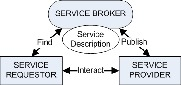
\includegraphics[width=0.8\textwidth]{soaDiagram}}
\caption{El dibujito basico.}
\label{fig:spontaneous}
\end{figure}

%%%%%%%%%%%%%% Bibliografia %%%%%%%%%%%%%%%

%\bibliographystyle{alpha}  % Eliminarlo al compilar el documento maestro, ponerlo para compilarlo separado
%\bibliography{p2pcomputing}%,gprop,mmitchell,zmich,hilera,fjmm,ripley,rbeale,jhertz,mag}       % Eliminarlo al compilar el documento maestro, ponerlo para compilarlo separado

%\end{document}             % Eliminarlo al compilar el documento maestro, ponerlo para compilarlo separado
\include{partes/3soaea}
\include{partes/4implementation}
\include{partes/5selfsizing}
\include{partes/6conclusions}
\include{partes/7conclusiones}
%%\documentclass[12pt,a4paper,twoside]{book} 
\usepackage[spanish]{babel} % de pedro
\usepackage{graphics,graphicx,epsfig,color,float,afterpage,fancyheadings,subfigure,moreverb,alltt} % de pedro
\usepackage[latin1]{inputenc} % tildes de pedro

\usepackage{algorithm}
\usepackage{algorithmic}

\usepackage{rotating}
\usepackage{url}

%% Esta letra se convierte mejor a pdf que la normal
\usepackage{ae}

%%% Para las fuentes matemticas
\usepackage{amsfonts}

\usepackage{subfigure}

\usepackage{pstricks} % para los dibujos del da
\usepackage{lscape} % para las pginas en horizontal
\usepackage{portland} % para las pginas en horizontal
\usepackage{supertabular} % para las tablas de ms de una pgina
\usepackage{tabularx} % para las tablas del tipo tabularx
%\usepackage{glossary}
%\documentclass[a4paper,spanish,12pt]{book} % esto es de gustavo
%\usepackage{amsmath,amsfonts}   % underset mathbb
%\usepackage{authordate1-4}      % bib style
%\usepackage{epsfig}     % eps
\usepackage{epic}           % graficos
%\usepackage{eepic}           % graficos
\usepackage{curvesls}           % curvas
\usepackage{amssymb}
%\usepackage{fancyheadings}  % encabezados
%\usepackage{hhline}             % hhline
%\usepackage[latin1]{inputenc}   % tildes
%\usepackage{makeidx}        % ndices
%\usepackage{setspace}           % interlinea
%\usepackage[spanish]{babel} % espaol

%%%%%%%%%%%%%%%%%%%%%%%%%%%%%%%%%%%%%%%%%%%%%%%%%%%%%%%%%%%%%%%%%%%%%%%%%%%%%%%

\author{juanlu}
\title{Tesis de Juan Lus Jimnez Laredo}




\newcommand{\fecha}{\footnotesize{[ Impreso: \the\day-\ifcase\month\or
    Ene\or Feb\or Mar\or Abr\or May\or Jun\or Jul\or Ago\or Sep\or
      Oct\or Nov\or Dic\fi-\the\year ]}}

\newcommand{\N}{\mathbb{N}}

%% Para corregir las cabeceras largas
\newcommand{\cabecera}[2]{
\markright{\ref{#1}. \hspace{0.1ex} \MakeUppercase{#2}}}


%\pagestyle{headings}
%\renewcommand{\chaptermark}[1]{\markboth{\fecha \\ \\ #1}{}}
%\renewcommand{\sectionmark}[1]{\markright{#1 \\ \\ \fecha}}
%\addtolength{\headheight}{2.5pt}



%\lhead[\it\thechapter]{\sl\rightmark}
%\rhead[\rm\leftmark]{\it\thesection}
%\rfoot[]{\thepage}
%\cfoot[]{}
%\lfoot[\thepage]{}

%\thispagestyle{plain}

\setcounter{secnumdepth}{3}
\setcounter{tocdepth}{3}

%\renewcommand{\baselinestretch}{1.2}
%\setlength{\parskip}{0.8ex}

\newtheorem{theorem}{\sf Teorema}
\newtheorem{lemma}{\sf Lema}

\newcommand{\rem}[1]{\S\iffalse #1 \fi}
\newcommand{\cur}[1]{ {\it #1\/} }
\newcommand{\crcl}[1]{#1\kern-9pt\raise1pt\hbox{$\bigcirc$}}
\newcommand{\evag}{{\sf EvAg}}
\newcommand{\evagp}{{\sf EvAg.}}
\newcommand{\evags}{{\sf EvAgs}}
\newcommand{\evagsp}{{\sf EvAgs.}}

\newcommand{\prog}[2] {
   \small
   \begin{minipage}[t]{75mm} {\tt #1}  \end{minipage}
   \begin{minipage}[t]{60mm} {#2}      \end{minipage}
   \\
}
\newcommand{\prg}[2] { {\tt #1} & {\sf #2} \\}

\newcommand{\wmfspecial}[4]{
   \begin{figure}[h]
   \centerline{\psfig{figure=#1,height=#2}}
   \caption{#3}   \label{#4}
   \end{figure}
}                   % USO: \wmfspecial{nombre.eps}{altura}{leyenda}{etiqueta}

\def\stackunder#1#2{\mathrel{\mathop{#2}\limits_{#1}}}

\def\marco #1#2#3#4{\centerline{       % USO: \marco{.1}{10}{124mm}
  \vbox{\hrule height #1pt%
  \hbox{\vrule width #1pt\kern #2pt%
  \vbox{\kern #2pt%
  \vbox{\hsize #3\noindent #4}%
  \kern #2pt}%
  \kern #2pt\vrule width #1pt}%
  \hrule height0pt depth #1pt}} }


\newcommand{\symnote}[2]{\symbolnote{#1}{#2}}

\newfont{\bi}{cmbxti10 scaled\magstep1}       % bf + it


%% Ruta de las figuras
\graphicspath{{../figuras/}}


\begin{document}
           % Eliminarlo al compilar el documento maestro, ponerlo para compilarlo separado

%%%%%%%%%%%%%%%%%%%%%%%%%%%%%%%%%%%%%%%%%%%%%%%%%%%%%%%%%%%%%%%%%%%%%%%%%%%%%%%
%%                                                                           %%
%%                             Tesis Doctoral:                               %%
%%                         Juan Luis Jimenez Laredo                          %%
%%%%%%%%%%%%%%%%%%%%%%%%%%%%%%%%%%%%%%%%%%%%%%%%%%%%%%%%%%%%%%%%%%%%%%%%%%%%%%%
\appendix
\cabecera{cap:appendixA}{Appendix A: Tuning of the Cache size parameter }
\chapter{\textit{Tuning of the Cache size parameter}}
\label{cap:appendixA}
\cabecera{cap:appendixA}{Appendix A: Tuning of the Cache size parameter }



Parallelising an EA implies the use of new parameters to control issues such as migration rates or the topology management. These new components drastically increase the complexity for the fine-tuning of the algorithm. In this sense, Cant\'u-Paz in \cite{cantu99:topologies} and Hidalgo and Fernandez in \cite{Fernandez:balancing} analyse up to seven  parameters derived from the parallelisation using islands. Within the \evag model instead, newscast simplifies all the decision making for the parallelisation by tuning  a single parameter, the cache size. The cache acts as a routing table  in which every peer holds a list of neighbours peers. Therefore, the cache size represents the maximum number of connections (edges) that a peer could have. Taking into account the recommendations of Jelasity et al. in \cite{jelasity:gossip}, the cache size has to be much smaller than the number of peers in order to get small-world features such as a small network diameter or a high clustering coefficient. 

Given the importance of the parameter, this appendix tries to calibrate an adequate cache size for the problems under study in this thesis. To this aim, we  measure the influence of different cache and population sizes on the algorithm performance when tackling a 4-trap instance. As will be shown, results indicate that success rates of the algorithm remain constant independently of the different cache sizes. This fact points to the robustness of the parallel model and helps decision making. Any cache size guaranteeing a small-world topology will produce equivalent performances.

Table \ref{table:appendix:parameters} summarizes the settings for the experiments in which eleven different cache sizes and two different population sizes have been tested.




\begin{table}[htbp]
\centering
{\scriptsize
\begin{tabular}{r c}
\hline
\multicolumn{2}{l}{\textbf{Problem instance}}\\
\hline
Problem & 4-trap\\
Chromosome length & 36\\
\\
\multicolumn{2}{l}{\textbf{\evag settings}}\\
\hline
Population size & 400, 600 individuals \\
Selection & Binary Tournament\\
Recombination & Uniform Crossover, $p_c = 1.0$ \\
Max. Eval. & 500000\\
\\
\multicolumn{2}{l}{\textbf{Newscast settings}}\\
\hline
 $Cache_{size}$ & 10,14,18,22,26,30,34,38,42,46,50\\ 

\end{tabular}
}
\caption{Settings for the experiments.\label{table:appendix:parameters}}
\end{table}




%%%%%%%%%%%%%%%%%%%%%%%%%%%%%%%%%%%%%%%%%%%%%%%%%%%%%%%%%%%%%%
\section{Analysis of Results}

Figure \ref{fig:cache:4trap} shows the SR and AES of the \evag 
model when tackling the 4-trap instance using different cache and population sizes. It can be observed how the population size has an impact on the algorithm performance while the cache size does not. 

The P2P EA is sensitive to the population size since the algorithm converges with a SR $\sim 0.85$ for $N=600$ while it decreases to $\sim 0.52$ for $N=400$. Nevertheless, results for different cache sizes move around the same SRs and AES. This way, neither the algorithm quality nor the execution time seems to be altered when using different settings for the cache size.

%The larger population size improves the quality of the solutions increasing, in turn, the computational effort. However, the cache size parameter does not seem to alter the algorithm performance neither in terms of quality (SR) nor execution-times (AES).

  

 This fact translates into the robustness of the \evag model with respect to such a parameter and is specially remarkable from the point of view of tuning the parameters of the algorithm. Choosing any cache size within the range $[10\dots50]$ will not alter the \evag performance.

\begin{figure}[htbp]
\centerline{
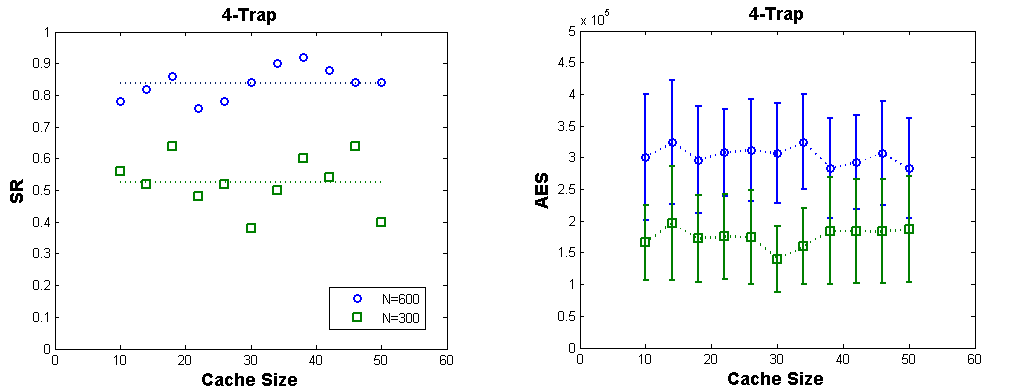
\includegraphics[width=\textwidth]{4trapcache}
}
\caption{Success Rate of the \evag model ({\em left}) and Average Evaluation to Solution with standard deviation ({\em right})
for a 4-trap instance using population sizes of $N=400$ and $N=600$. Averaged values for the different cache sizes in dotted lines.}
\label{fig:cache:4trap}
\end{figure}





%\bibliographystyle{alpha}  % Eliminarlo al compilar el documento maestro, ponerlo para compilarlo separado
%\bibliography{evagperformance,pea,p2pcomputing,model}% Eliminarlo al compilar el documento maestro, ponerlo para compilarlo separado

%\end{document}             % Eliminarlo al compilar el documento maestro, ponerlo para compilarlo separado

%%\documentclass[12pt,a4paper,twoside]{book} 
\usepackage[spanish]{babel} % de pedro
\usepackage{graphics,graphicx,epsfig,color,float,afterpage,fancyheadings,subfigure,moreverb,alltt} % de pedro
\usepackage[latin1]{inputenc} % tildes de pedro

\usepackage{algorithm}
\usepackage{algorithmic}

\usepackage{rotating}
\usepackage{url}

%% Esta letra se convierte mejor a pdf que la normal
\usepackage{ae}

%%% Para las fuentes matemticas
\usepackage{amsfonts}

\usepackage{subfigure}

\usepackage{pstricks} % para los dibujos del da
\usepackage{lscape} % para las pginas en horizontal
\usepackage{portland} % para las pginas en horizontal
\usepackage{supertabular} % para las tablas de ms de una pgina
\usepackage{tabularx} % para las tablas del tipo tabularx
%\usepackage{glossary}
%\documentclass[a4paper,spanish,12pt]{book} % esto es de gustavo
%\usepackage{amsmath,amsfonts}   % underset mathbb
%\usepackage{authordate1-4}      % bib style
%\usepackage{epsfig}     % eps
\usepackage{epic}           % graficos
%\usepackage{eepic}           % graficos
\usepackage{curvesls}           % curvas
\usepackage{amssymb}
%\usepackage{fancyheadings}  % encabezados
%\usepackage{hhline}             % hhline
%\usepackage[latin1]{inputenc}   % tildes
%\usepackage{makeidx}        % ndices
%\usepackage{setspace}           % interlinea
%\usepackage[spanish]{babel} % espaol

%%%%%%%%%%%%%%%%%%%%%%%%%%%%%%%%%%%%%%%%%%%%%%%%%%%%%%%%%%%%%%%%%%%%%%%%%%%%%%%

\author{juanlu}
\title{Tesis de Juan Lus Jimnez Laredo}




\newcommand{\fecha}{\footnotesize{[ Impreso: \the\day-\ifcase\month\or
    Ene\or Feb\or Mar\or Abr\or May\or Jun\or Jul\or Ago\or Sep\or
      Oct\or Nov\or Dic\fi-\the\year ]}}

\newcommand{\N}{\mathbb{N}}

%% Para corregir las cabeceras largas
\newcommand{\cabecera}[2]{
\markright{\ref{#1}. \hspace{0.1ex} \MakeUppercase{#2}}}


%\pagestyle{headings}
%\renewcommand{\chaptermark}[1]{\markboth{\fecha \\ \\ #1}{}}
%\renewcommand{\sectionmark}[1]{\markright{#1 \\ \\ \fecha}}
%\addtolength{\headheight}{2.5pt}



%\lhead[\it\thechapter]{\sl\rightmark}
%\rhead[\rm\leftmark]{\it\thesection}
%\rfoot[]{\thepage}
%\cfoot[]{}
%\lfoot[\thepage]{}

%\thispagestyle{plain}

\setcounter{secnumdepth}{3}
\setcounter{tocdepth}{3}

%\renewcommand{\baselinestretch}{1.2}
%\setlength{\parskip}{0.8ex}

\newtheorem{theorem}{\sf Teorema}
\newtheorem{lemma}{\sf Lema}

\newcommand{\rem}[1]{\S\iffalse #1 \fi}
\newcommand{\cur}[1]{ {\it #1\/} }
\newcommand{\crcl}[1]{#1\kern-9pt\raise1pt\hbox{$\bigcirc$}}
\newcommand{\evag}{{\sf EvAg}}
\newcommand{\evagp}{{\sf EvAg.}}
\newcommand{\evags}{{\sf EvAgs}}
\newcommand{\evagsp}{{\sf EvAgs.}}

\newcommand{\prog}[2] {
   \small
   \begin{minipage}[t]{75mm} {\tt #1}  \end{minipage}
   \begin{minipage}[t]{60mm} {#2}      \end{minipage}
   \\
}
\newcommand{\prg}[2] { {\tt #1} & {\sf #2} \\}

\newcommand{\wmfspecial}[4]{
   \begin{figure}[h]
   \centerline{\psfig{figure=#1,height=#2}}
   \caption{#3}   \label{#4}
   \end{figure}
}                   % USO: \wmfspecial{nombre.eps}{altura}{leyenda}{etiqueta}

\def\stackunder#1#2{\mathrel{\mathop{#2}\limits_{#1}}}

\def\marco #1#2#3#4{\centerline{       % USO: \marco{.1}{10}{124mm}
  \vbox{\hrule height #1pt%
  \hbox{\vrule width #1pt\kern #2pt%
  \vbox{\kern #2pt%
  \vbox{\hsize #3\noindent #4}%
  \kern #2pt}%
  \kern #2pt\vrule width #1pt}%
  \hrule height0pt depth #1pt}} }


\newcommand{\symnote}[2]{\symbolnote{#1}{#2}}

\newfont{\bi}{cmbxti10 scaled\magstep1}       % bf + it


%% Ruta de las figuras
\graphicspath{{../figuras/}}


\begin{document}
           % Eliminarlo al compilar el documento maestro, ponerlo para compilarlo separado

%%%%%%%%%%%%%%%%%%%%%%%%%%%%%%%%%%%%%%%%%%%%%%%%%%%%%%%%%%%%%%%%%%%%%%%%%%%%%%%
%%                                                                           %%
%%                             Tesis Doctoral:                               %%
%%                         Juan Luis Jimenez Laredo                          %%
%%%%%%%%%%%%%%%%%%%%%%%%%%%%%%%%%%%%%%%%%%%%%%%%%%%%%%%%%%%%%%%%%%%%%%%%%%%%%%%

\cabecera{cap:appendixB}{Appendix B: Numerical Results}
\chapter{\textit{Numerical Results}}
\label{cap:appendixB}
\cabecera{cap:appendixB}{Appendix B: Numerical Results}

In this appendix, numerical results for the scalability analysis of the different test cases are presented. The aim of providing such values is to allow a numerical comparison of results in addition to the respective one of the graphs depicted in chapter  \ref{cap:evagperformance}. As saw in Section \ref{sec:metrics}, central position values (e.g. the mean) are not representative of the distributions on the computational efforts since they do not keep normality conditions. Therefore, the following tables provide the first, second and third quartiles of the distributions as values of reference.


%%%%%%%%%%%%%%%%%%%%%%%%%%%%%%%%%%%%%%%%%%%%%%%%%%%%%%%%%%%%%%
\begin{sidewaystable}[htbp]
%\begin{table*}[htbp]
\centering
{\tiny
\begin{tabular}{c|c c c c|c c c c|c c c c|}

{\it Problem}&\multicolumn{4}{|c|}{GGA}&\multicolumn{4}{|c|}{SSGA}&\multicolumn{4}{|c|}{EvAg}\\
{\it Instance}&\multicolumn{4}{|c|}{}&\multicolumn{4}{|c|}{}&\multicolumn{4}{|c|}{}\\
\hline
\multicolumn{13}{c}{{\it Selectorecombinative}}\\
\hline
2-Trap&N&$Q_1$&$Q_2$&$Q_3$&N&$Q_1$&$Q_2$&$Q_3$&N&$Q_1$&$Q_2$&{\it {\bf $Q_3$}}\\
\hline
12&60&258&365&426&67 &182 &220 &296 &30&187&240&330\\
24&135&1495&1767&2136& 165 &886  &974  &1086  &48&828&960&1092\\
36&170&2735&2906&3077& 240 &1813  &1913  &2052  &75&1725&1875&2156\\
48&250&5019&5395&5772& 300 & 2743 &2906   & 3066  &90&2700&2970&3577\\
{\it {\bf 60}}&320&7382&7832&8024& 300 & 3318 & 3530 & 3801 & 135&4590&4927&5535\\
\hline
3-Trap&N&$Q_1$&$Q_2$&$Q_3$&N&$Q_1$&$Q_2$&$Q_3$&N&$Q_1$&$Q_2$&{\bf $Q_3$}\\
\hline
12&360&811&1443&2526&165 &472 & 637 & 783  &48&336&528&948\\
24&3120&53056&56177&64759&660  &4678  &5453  &6034  &105&2861&4200&5670\\
36&5280&142586&153148&163710& 960 & 11346 & 12257 & 13596 &195&10383&12772&15990\\
48&7680&268834&284196&299558& 1440 & 23024 & 24810 & 26182 &390&26227&28665&33345\\
{\bf 60}&11520&472360&483881&506923& 1920 & 37986 & 39553& 42100 & 480&39240&44880& 49920\\
\hline
4-Trap&N&$Q_1$&$Q_2$&$Q_3$&N&$Q_1$&$Q_2$&$Q_3$&N&$Q_1$&$Q_2$&{\bf $Q_3$}\\
\hline
12& 2880&2880 &2880 &5761  &960  &1502  &2651  &5470 &60&510&1110&2880\\
16& 53760  & 53760 & 53760 & 107521 & 3120& 10475& 18128 &32272 &-&-&-&-\\
24&-&-&-&-&-&-&-&-&225&33862&42525&55293\\
{\bf 36}&-&-&-&-&-&-&-&-&{\bf 600}&267750&314400&{\bf 393000}\\
\hline
\multicolumn{13}{c}{{\it Using a mutation rate of $\frac{1}{L}$}}\\
\hline
2-Trap&N&$Q_1$&$Q_2$&$Q_3$&N&$Q_1$&$Q_2$&$Q_3$&N&$Q_1$&$Q_2$&{\it {\bf $Q_3$}}\\
\hline
12&*&304 &426 &593 &* &214 &305 &374 &*&210 &300 &420 \\
24&*&2039 &2447 &2885 &* &1080 &1244 &1418 &*&1008 &1128 &1248 \\
36&*&4103 &4616 &5300 &* &2270 &2497 &2736 &*&2175 &2475 &2737 \\
48&*&7278 &7780 &8031 &* &3543 &3709 &3880 &*&3330 &3690 &4320 \\
60&*&10592 &11232 &11876 &*&4283& 4449& 4722&*& 5535& 6075&6581\\
\hline
3-Trap&N&$Q_1$&$Q_2$&$Q_3$&N&$Q_1$&$Q_2$&$Q_3$&N&$Q_1$&$Q_2$&{\bf $Q_3$}\\
\hline
12&*&1082 &1443 &2887 &* &456 &599 &826 &*&432 &528 &720 \\
24&*&86606 &99871 &109234 &* &5925 &6631 &7454 &*&3701 &4830 &6195 \\
36&*&237644 &253487 &279892 &* &15346 &16638 &18613 &*&11700 &15404 &17842 \\
48&*&422454 &445497 & 466619&* &29021 &30570 &33498 &*&32955 &37050 &43582 \\
60&*&725822 &748864 &794948 &* &48089 &51137 &54229 &*&54360 &61200 &66480 \\
\hline
4-Trap&N&$Q_1$&$Q_2$&$Q_3$&N&$Q_1$&$Q_2$&$Q_3$&N&$Q_1$&$Q_2$&{\bf $Q_3$}\\
\hline
12&*&2880 &2880 &5761 &* &1526 &2510 &4517 &*&675 &1950 &5205\\
16&*&53760 &53760 &107521 &* &11055 &21898 &33353 &*&-&-&-\\
24&*&-&-&-&*&-&-&-&*&32456 &51750 &69525 \\
36&*&-&-&-&*&-&-&-&*&434550 &531900 &655350 \\
\hline

\end{tabular}
}
\caption{Test-Case 1: Number of evaluations to solution in $Q_1$, $Q_2$ and $Q_3$ for different trap functions and chromosome lengths $L$. Population sizes of the problem instances are estimated by bisection using a selectorecombinative GA.\label{table:numericalresultstestcase1}}
%\end{table*}
\end{sidewaystable}
%%%%%%%%%%%%%%%%%%%%%%%%%%%%%%%%%%%%%%%%%%%%%%%%%%%%%%%%%%%%%%


%%%%%%%%%%%%%%%%%%%%%%%%%%%%%%%%%%%%%%%%%%%%%%%%%%%%%%%%%%%%%%
\begin{sidewaystable}[htbp]
%\begin{table*}[htbp]
\centering
{\tiny
\begin{tabular}{c|c c c c|c c c c| c c c c|}

{\it Problem}&\multicolumn{4}{|c|}{\evag}&\multicolumn{4}{|c|}{\evag}&\multicolumn{4}{|c|}{\evag}\\
{\it Instance}&\multicolumn{4}{|c|}{Ring}&\multicolumn{4}{|c|}{Watts-Strogatz}&\multicolumn{4}{|c|}{Newscast}\\
\hline
2-Trap&N&$Q_1$&$Q_2$&$Q_3$&N&$Q_1$&$Q_2$&$Q_3$&N&$Q_1$&$Q_2$&{\it {\bf $Q_3$}}\\
\hline
12&30&210&255&330&30&187&240&330&30&187&240&330\\
24&37&999&1628&2136&41&738&861&1055&48&828&960&1092\\
36&41&2870&3567&4612&60&1440&1620&1980&75&1725&1875&2156\\
48&52&5226&7748&9451&97&2910&3492&3880&90&2700&2970&3577\\
{\it {\bf 60}}&60&11010&14850&17460&90&3600&3920&4410&{\it {\bf 135}}&4590&4927&{\it {\bf 5535}}\\
\hline
3-Trap&N&$Q_1$&$Q_2$&$Q_3$&N&$Q_1$&$Q_2$&$Q_3$&N&$Q_1$&$Q_2$&{\bf $Q_3$}\\
\hline
1241&369&738&1588&41&246&410&697&48&336&528&948\\
24&60&6840&11730&17220&67&2646&3785&5845&105&2861&4200&5670\\
36&75&35943&58800&78393&135&8741&11542&16436&195&10383&12772&15990\\
48&90&138172&184005&272182&195&21206&37927&48701&390&26227&28665&33345\\
{\bf 60}&135&570780&770850&1203491&270&62167&94905&138307&{\bf 480}&39240&44880&{\bf 49920}\\
\hline
4-Trap&N&$Q_1$&$Q_2$&$Q_3$&N&$Q_1$&$Q_2$&$Q_3$&N&$Q_1$&$Q_2$&{\bf $Q_3$}\\
\hline
12&90&990&2565&7470&60&630&1500&2775&60&510&1110&2880\\
24&90&63922&98055&149355&150&27412&39150&48075&225&33862&42525&55293\\
{\bf 36}&225&957206&1304325&1989056&300&158325&193500&232650&{\bf 600}&267750&314400&{\bf 393000}\\
\hline

\end{tabular}
}
\caption{Test-Case 2: Number of evaluations to solution in $Q_1$, $Q_2$ and $Q_3$ for different trap functions and chromosome lengths $L$. Population sizes of the problem instances are estimated by bisection using a selectorecombinative GA..\label{table:numericalresultstestcase2}}
%\end{table*}
\end{sidewaystable}
%%%%%%%%%%%%%%%%%%%%%%%%%%%%%%%%%%%%%%%%%%%%%%%%%%%%%%%%%%%%%%



%%%%%%%%%%%%%%%%%%%%%%%%%%%%%%%%%%%%%%%%%%%%%%%%%%%%%%%%%%%%%%
\begin{sidewaystable}[htbp]
%\begin{table*}[htbp]
\centering
{\tiny
\begin{tabular}{c|c c c c|c c c c| c c c c|}

{\it Problem}&\multicolumn{4}{|c|}{Churn}&\multicolumn{4}{|c|}{Churn}&\multicolumn{4}{|c|}{No Churn}\\
{\it Instance}&\multicolumn{4}{|c|}{$\lambda = 400$}&\multicolumn{4}{|c|}{$\lambda = 2500$}&\multicolumn{4}{|c|}{ }\\
\hline
2-Trap&N&$Q_1$&$Q_2$&$Q_3$&N&$Q_1$&$Q_2$&$Q_3$&N&$Q_1$&$Q_2$&{\it {\bf $Q_3$}}\\
\hline
12&40 &142 &264 &392               &40 &135 &258 &401        &30&187&240&330\\
24&60 &805 &952 &1150               &65 &752 &956 &1120        &48&828&960&1092\\
36&100 &1705 &2019 &2482               &110 &1895 &2146 &2642        &75&1725&1875&2156\\ 
48&130 &2815 &3007 &3625               &130 &2915 &3309 &3825        &90&2700&2970&3577\\
{\it {\bf 60}}&200 &4901 &5149 &6012   &180 &4870 &5161 &6030        &{\it {\bf 135}}&4590&4927&{\it {\bf 5535}}\\
\hline
3-Trap&N&$Q_1$&$Q_2$&$Q_3$&N&$Q_1$&$Q_2$&$Q_3$&N&$Q_1$&$Q_2$&{\bf $Q_3$}\\
\hline
12 &65 &422 &749 &1050          &65 &437 &653 &1120           &48&336&528&948\\
24 &150 &2980 &4014 &5723          &120 &3008 &4203 &5432           &105&2861&4200&5670\\
36 &360 &8026 &14955 &21712          &300 &10702 &13665 &16722           &195&10383&12772&15990\\
48 &720 &28334 &33687 &38137          &440 &22170 &27310 &31543           &390&26227&28665&33345\\
{\bf 60}&1120 &56971 &61970 &69790     &720 &46713 &52646 &60910           &{\bf 480}&39240&44880&{\bf 49920}\\
\hline
4-Trap&N&$Q_1$&$Q_2$&$Q_3$&N&$Q_1$&$Q_2$&$Q_3$&N&$Q_1$&$Q_2$&{\bf $Q_3$}\\
\hline
12&120 &2890 &3349 &5314             &110 &1080 &2733 &4712           &60&510&1110&2880\\
24&320 &38278 &49862 &64120             &320 &35738 &52912 &63615           &225&33862&42525&55293\\
{\bf 36}&1280 &28764 &367377 &451320       &880 &260914 &385931 &498027           &{\bf 600}&267750&314400&{\bf 393000}\\
\hline

\end{tabular}
}
\caption{Test-Case 3: Number of evaluations to solution in $Q_1$, $Q_2$ and $Q_3$ for different trap functions and chromosome lengths $L$. Population sizes of the problem instances are estimated by bisection using a selectorecombinative GA.\label{table:numericalresultstestcase3}}
%\end{table*}
\end{sidewaystable}
%%%%%%%%%%%%%%%%%%%%%%%%%%%%%%%%%%%%%%%%%%%%%%%%%%%%%%%%%%%%%%






%\bibliographystyle{alpha}  % Eliminarlo al compilar el documento maestro, ponerlo para compilarlo separado
%\bibliography{evagperformance,pea,p2pcomputing,model}% Eliminarlo al compilar el documento maestro, ponerlo para compilarlo separado

%\end{document}             % Eliminarlo al compilar el documento maestro, ponerlo para compilarlo separado

%%%%%%%%%%%%%%%%%%%%%%%%%%%%%%%%%%%%%%%%%%%%%%%%%%%%%%%%%%%%%%%%%%%%%%%%%%%%%%%
%%                                                                           %%
%%                               Bibliografa                                %%
%%                                                                           %%
%%%%%%%%%%%%%%%%%%%%%%%%%%%%%%%%%%%%%%%%%%%%%%%%%%%%%%%%%%%%%%%%%%%%%%%%%%%%%%%
\backmatter
%%%%%%%%%%%%%%%%%%%%%%%%%%%%%%%%%%%%%%%%%%%%%%%%%%%%%%%%%%%%%%%%%%%%%%%%%%%%%%%
%%                                                                           %%
%%                               Bibliografa                                %%
%%                                                                           %%
%%%%%%%%%%%%%%%%%%%%%%%%%%%%%%%%%%%%%%%%%%%%%%%%%%%%%%%%%%%%%%%%%%%%%%%%%%%%%%%

\bibliographystyle{plain}
\bibliography{partes/p2pcomputing,partes/pea,partes/model,partes/methodology,partes/evagperformance}

%%%%%%%%%%%%%%%%%%%%%%%%%%%%%%%%%%%%%%%%%%%%%%%%%%%%%%%%%%%%%%%%%%%%%%%%%%%%%%%


\end{document}
